\documentclass[../../topologia_algebraica]{subfiles}
\begin{document}
\section{Cobordismo}\label{sec:cobordismo}

\subsection{Conos}

\begin{defin}
  El \emph{cono} de un espacio $X$ se define como:
  \[
    CX := (X\times I)/_{X\times\{1\}}
  \] 

  Si el espacio es basado, ie $(X,x)$, entonces su cono se define como
  \[
    C(X,x):=(X\times I)/_{(X\times \{1\})\cup(\{x\}\times I)}
  \]
\end{defin}

 Ve la figura \ref{fig:cono_circulo}.

\begin{nota}
  Observa que el cono viene equipado de una inclusi\'on natural $\imath:X\hookrightarrow CX$ con la
  regla $x\mapsto [x,0]$.
\end{nota}

\import{\directory}{ejercicios/36} %%%%%%%%%%%%%%%%%%%%%%%%%%%%%%%%%%%%%%%%%%%%%%%%%%%%%%%% EJERCICIO 36

\begin{lema}
  Sea $f:X\ra Y$ una funci\'on continua. $f$ es contraible si y s\'olo si $f$ se extiende a $CX$, es
  decir:
  \[
    f\simeq\cte \quad\iff\quad
    \begin{tikzcd}
      CX \arrow[dr,dashed,"\hat{f}"] & \\
      X \arrow[u,hook,"\imath"] \arrow[r,"f"'] & Y
    \end{tikzcd}
  \]
\end{lema}

\begin{proof}
\begin{enumerate}
  \item[($\then$)]
    Supongo que $f\simeq\cte$ mediante la homotop\'ia $H:X\times I\ra Y$. Como
    $H_1(x)=H(x,1)=\cte(x)=y_0\in Y$,
    entonces $H$ se factoriza a trav\'es de $(X\times I)/_{(X\times\{1\})}=CX$:
    \[
      \begin{tikzcd}
        X\times I \arrow[r,"H"] \arrow[d,two heads,"\nu"'] & Y \\
        CX \arrow[ur,dashed,"\bar{H}"'] &
      \end{tikzcd}
    \]
    Aqu\'i $\bar{H}$ es continua porque $H$ es continua y $\nu$ es una identificaci\'on.
  
    Como $H_0=f$, entonces $\bar{H}$ restringido a $X\times\{0\}$ es $f$, o equivalentemente
    $\bar{H}\circ\imath=f$. Por lo tanto $\bar{H}$ es la extensi\'on de $f$ buscada.
  \item[($\onlyif$)] Sea $\hat{f}:CX\ra Y$ una extensi\'on de $f$ y defino $H=\hat{f}\circ\nu$.
    Observa que
    \begin{eqnarray*}
      H(x,0)&=&\hat{f}[x,0]=\hat{f}(\imath(x))=f(x) \\
      H(x,1)&=&\hat{f}(*)=y_0
    \end{eqnarray*}
    donde $*=[x,1]\in CX$. Por lo tanto si $\cte$ es la funci\'on constante $y_0$, entonces
    $f\simeq \cte$.
\end{enumerate}
\end{proof}

\import{\directory}{ejercicios/37} %%%%%%%%%%%%%%%%%%%%%%%%%%%%%%%%%%%%%%%%%%%%%%%%%%% EJERCICIO 37

\begin{ejemplo}
  $C\Sn^1\approx\DD^2$
\begin{figure}[h] %%%%%%%%%%%%%%%%%%%%%%%%%%%%%%%%%%%%%%%%%%%%%%%%%%%%%%%%%%%%% FIGURA CONO_CIRCULO
    \centering\label{fig:cono_circulo}
    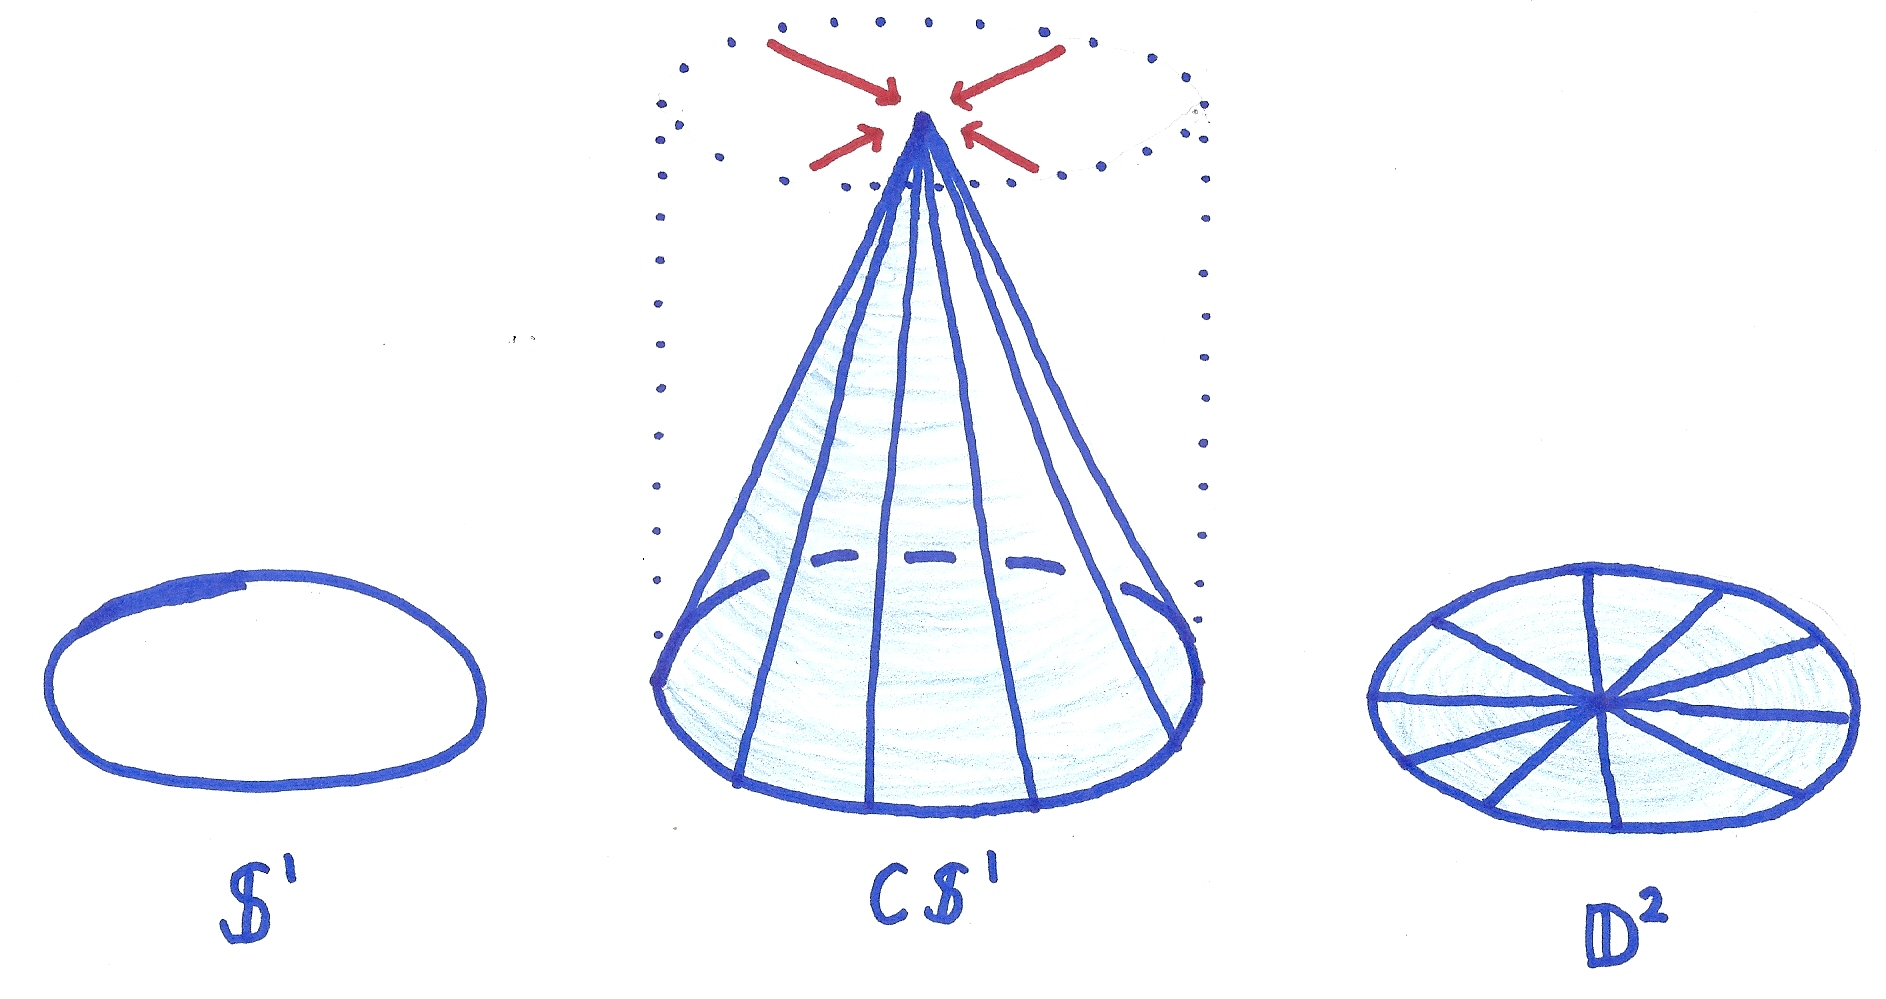
\includegraphics[scale=0.12]{cono_circulo}
\end{figure}%%%%%%%%%%%%%%%%%%%%%%%%%%%%%%%%%%%%%%%%%%%%%%%%%%%%%%%%%%%%%%%%%%%%%%%%%%%%%%%%%%%%%%%
\end{ejemplo}

\subsection{Clases de cobordismo}

Recuerda que si $N$ es una variedad suave, entonces $N\times I$ es una variedad suave con frontera
$\partial N \sqcup \partial N$. En particular
\[
  \partial(\Sn^n\times I)=(\Sn^n\times\{0\})\cup(\Sn^n\times\{1\})=\Sn^n \sqcup \Sn^n.
\]
Por lo
tanto una homotop\'ia $H:\Sn^n\times I\ra X$ entre dos funciones $\alpha,\beta:\Sn^n\ra X$ se
cumple
\[
  H|_{\Sn^n\times\{0\}}=\alpha \quad\text{y}\quad H|_{\Sn^n\times\{1\}}=\beta,
\]
donde podemos ver a los conjuntos $\Sn^n\times\{0\}$ y $\Sn^n\times\{1\}$ como la frontera de la
variedad $\Sn^n\times I$. En otras palabras puedo decir que $\alpha$ y $\beta$ est\'an relacionados
porque existe una variedad (ie. $\Sn^n\times I$) que tiene como frontera los dominios de $\alpha$
y $\beta$ , y una funci\'on $H$ definida sobre esa variedad que se restringe a $\alpha$ y a $\beta$.

Hago m\'as precisa esta idea:

\begin{defin}
  Sea $X$ un espacio topolo\'ogico. Si $M^n$ es una variedad suave y compacta, la pareja $(M,f)$
  es simplemente una funci\'on continua $f:M\ra X$ donde $M$ es considerada como subvariedad
  de alg\'un espacio euclideano. La \emph{relaci\'on de cobordismo} es la siguiente relaci\'on
  de equivalencia sobre tales parejas:
  \[
    (M^n,f)\sim(N^n,g) \quad\iff\quad
    \exists F:W^{n+1}\ra X;\;\text{continua tal que}\;\;
    \begin{cases}
      (i)& \partial W\cong M\sqcup N \\
      (ii)& F|_{M}=f \;\;\text{y}\;\; F|_{N}=g
    \end{cases}
  \]
  donde $W$ es una variedad suave, compacta, con frontera y de dimensi\'on $n+1$.
\end{defin}

Observa que s\'i es una relaci\'on de equivalencia. Claramente es sim\'etrica por definici\'on.
Es reflexiva porque $(M,f)\sim(M,f)$ mediante la variedad $W=M\times I$, que tiene frontera
$\partial W=M\sqcup M$, y la funci\'on $F:W\ra X$ definida por $F(x,t)=f(x)$.
La transitividad es dif\'icil de probar porque requiere un resultado muy fuerte de
topolog\'ia diferencial.

Sean $(M,f)\sim(N,g)$ y $(N,g)\sim(L,h)$ mediante $F:W\ra X$ y $G:V\ra X$ respectivamente.
Lo ideal es ``pegar'' $W$ y $V$ a lo largo de $N$:

\begin{figure}[ht] %%%%%%%%%%%%%%%%%%%%%%%%%%%%%%%%%%%%%%%%%%%%%%%%%%%% FIGURA BORDISMO_TRANSITIVIDAD
  \centering
  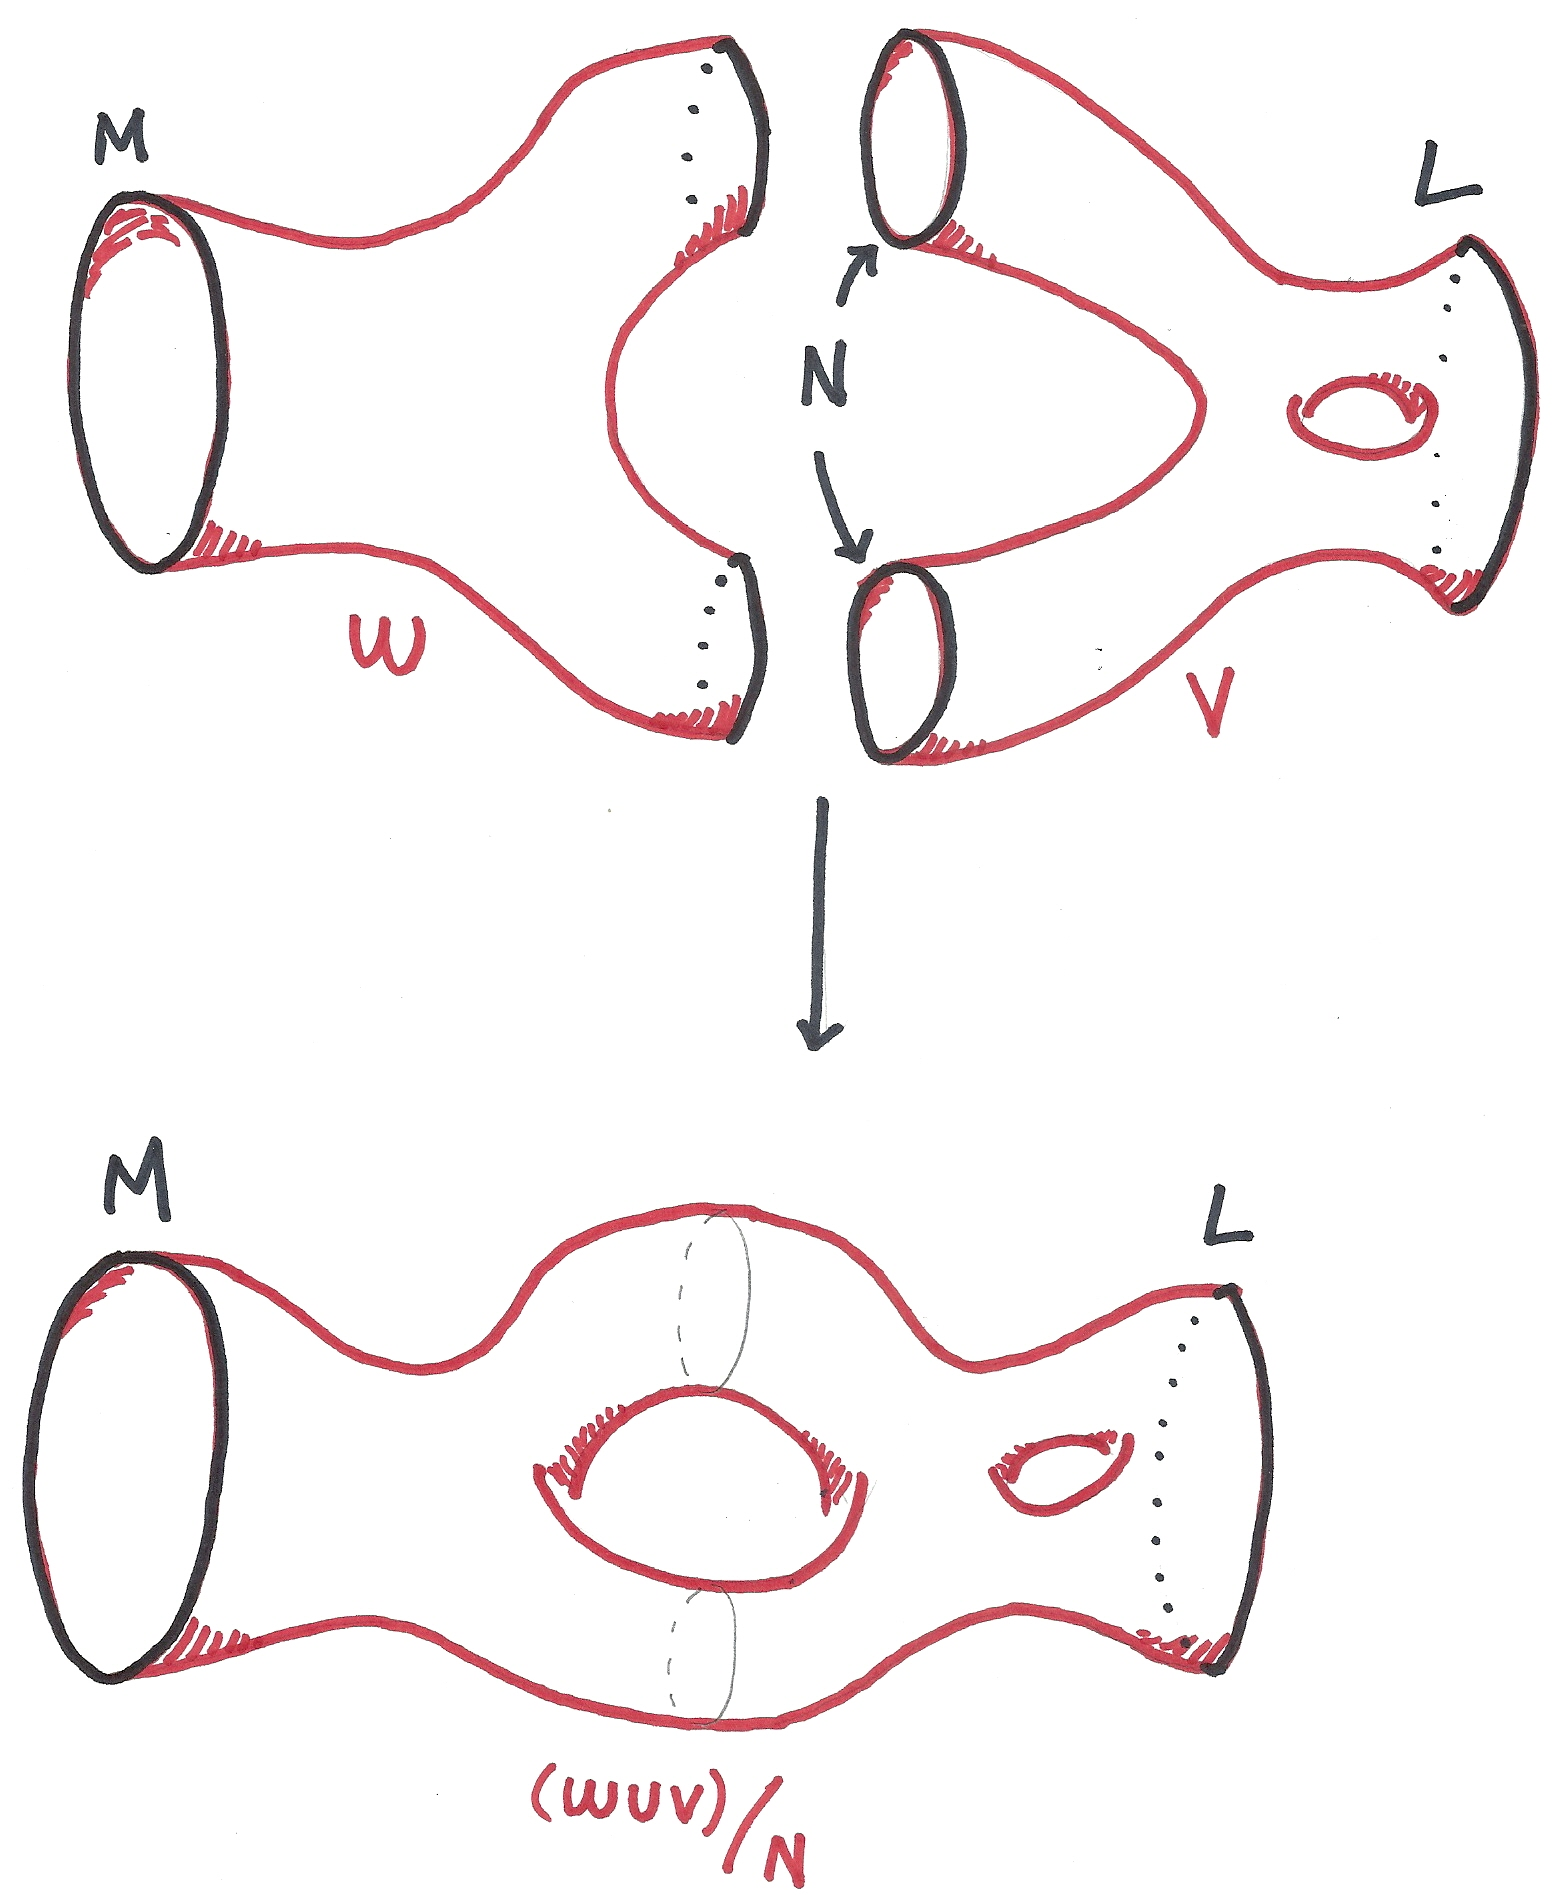
\includegraphics[scale=0.12]{bordismo_transitividad}
\end{figure} %%%%%%%%%%%%%%%%%%%%%%%%%%%%%%%%%%%%%%%%%%%%%%%%%%%%%%%%%%%%%%%%%%%%%%%%%%%%%%%%%%%%%%%%

\noindent para obtener la variedad suave $(W\cup V)/_N=:Y$, y as\'i poder definir
\[
  H:Y\ra X \quad\text{con}\quad  Y(x)=
  \begin{cases}
    F(x) & \text{si}\;\; x\in W \\
    G(x) & \text{si}\;\; x\in V
  \end{cases}
\]
que claramente implica que $(M,f)\sim (L,h)$. Lo \'unico que faltar\'ia probar es que $Y$
es una variedad suave, pero esto es consecuencia de los siguientes dos teoremas:

\begin{thm}
  Toda variedad suave $M$ con frontera tiene un collar, es decir existe un encaje
  $(\partial M\times [0,1))\hookrightarrow M$.
\end{thm}

\begin{thm}
  Sea $M$ una variedad suave con frontera, $\kappa:(\partial M\times[0,1))\ra M$ un collar
  y $\tau:\partial M\ra \partial M$ una funci\'on suave libre de puntos fijos tal que $\tau\circ\tau=\Id$.
  Entonces el espacio cociente $M/_{\tau}:=M/_{x\sim\tau(x)}$ tiene una \'unica estructura
  diferenciable tal que la inclusi\'on $M-\partial M \subset M/_{\tau}$ y la funci\'on
  \[
    \what{\kappa}:\frac{\partial M\times (-1,1)}{\tau\times(-\Id)} \lra \frac{M}{\tau}
    \quad\text{con}\quad \what{\kappa}[x,t]=
    \begin{cases}
      \kappa(x,t) &\text{si}\;\; t\geq 0 \\
      \kappa\big(\tau(x),-t \big) & \text{si}\;\; t\leq 0
    \end{cases}
  \]
  son encajes.
  \begin{figure}[ht] %%%%%%%%%%%%%%%%%%%%%%%%%%%%%%%%%%%%%%%%%%%%%%%%%%%%%%%%%%%%%%%%%%%% FIGURA COLLAR
    \centering
    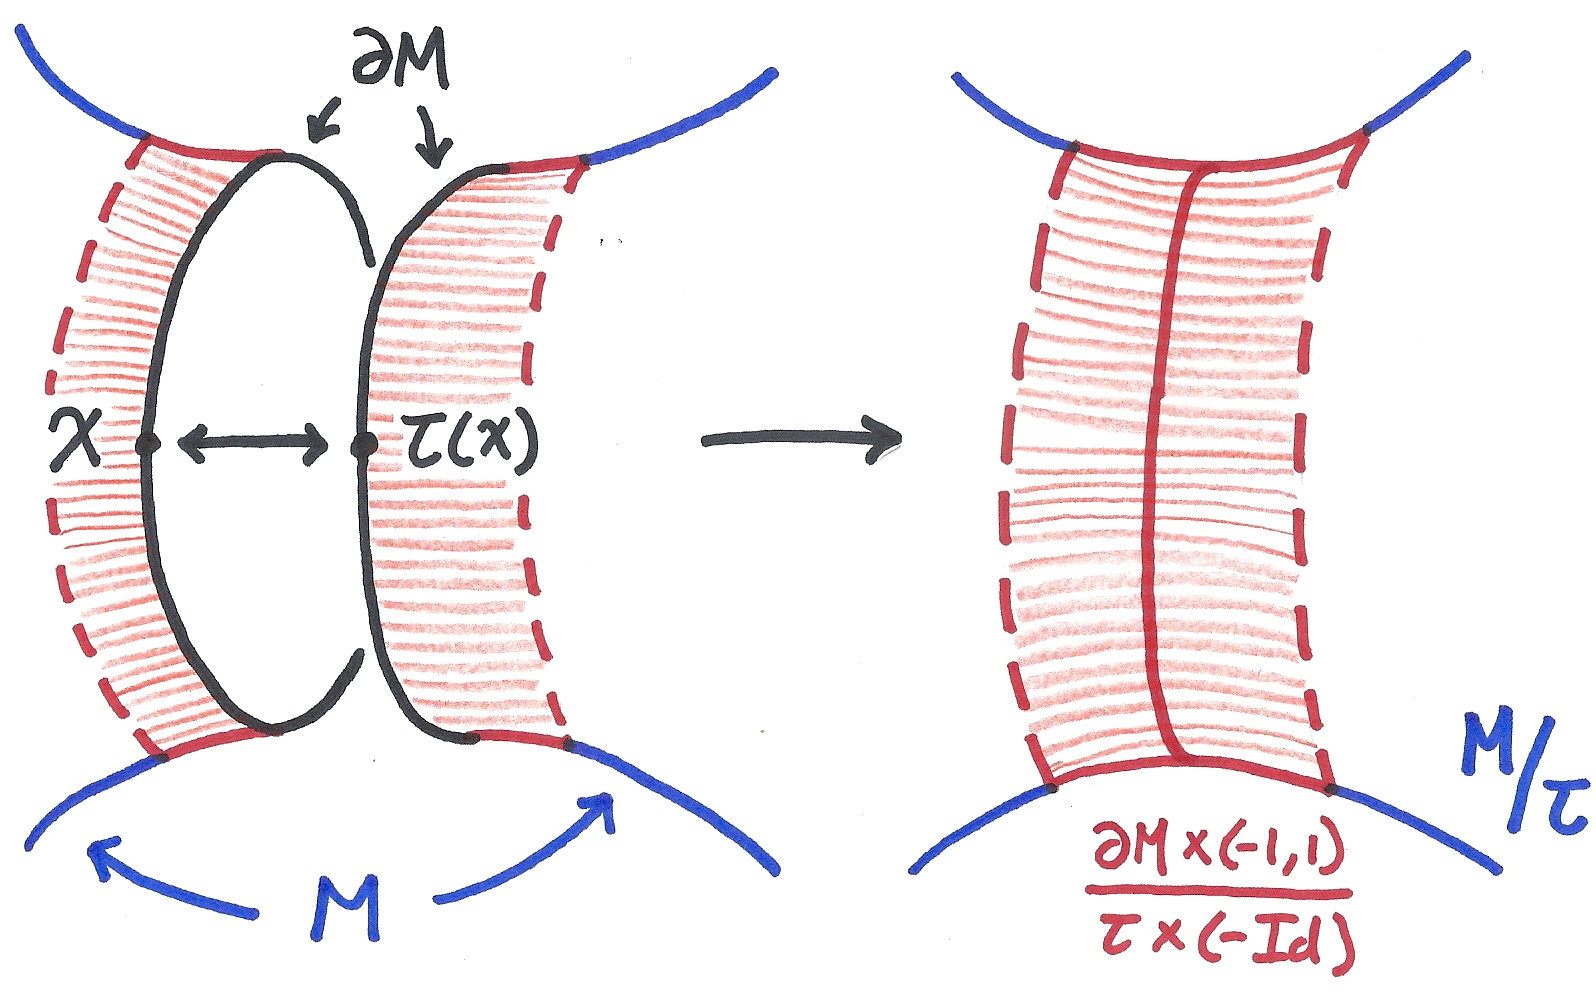
\includegraphics[scale=0.14]{collar}
  \end{figure} %%%%%%%%%%%%%%%%%%%%%%%%%%%%%%%%%%%%%%%%%%%%%%%%%%%%%%%%%%%%%%%%%%%%%%%%%%%%%%%%%%%%%%%%
\end{thm}

En palabras, este \'ultimo teorema dice que un collar permite identificar la frontera mediante
una involuci\'on sin puntos fijos de tal manera que el resto de la variedad (ie. $M-\partial M$)
no cambia y que los collares se pegan para dar un abierto de la variedad.

\begin{nota}
  Para la transitividad, estoy usando como variedad a $W\sqcup V$ y como involuci\'on $\tau:N\ra N$
  que simplemente cambia de copia de $N$ (observa que este no tiene puntos fijos porque el dominio
  y el contradominio de $tau$ son copias distintas de $N$ como subvariedad de $W\sqcup V$).
\end{nota}

\begin{defin}
  Al conjunto de clases de equivalencia $[M,f]$ donde $M$ es cerrada de dimensi\'on $n$ y $f:M\ra X$,
  se denota $\eta_n(X)$. Es un grupo abeliano con la suma
  \[
    [M,f]+[N,g]:=[M\sqcup N,f\sqcup g]
  \]
  y neutro $0=[\Sn^n,\cte]$.
\end{defin}

En efecto, $(M\sqcup\Sn^n,f\sqcup\cte)\sim(M,f)$ mediante la variedad $(M\times I)\sqcup \DD^{n+1}$,
que tiene frontera $M\sqcup (M\sqcup\Sn^n)$, y la funci\'on
\[
  F(x)=
  \begin{cases}
    f(y) &\text{si}\;\; x=(y,t)\in M\times I \\
    \cte &\text{si}\;\; x\in\DD^{n+1}
  \end{cases}.
\]

\begin{nota}
  Para evitar problemas conjuntistas, estoy asumiendo que todas las $n$-variedades cerradas est\'an
  encajadas en $\RR^{2n}$.
\end{nota}

\import{\directory}{ejercicios/38} %%%%%%%%%%%%%%%%%%%%%%%%%%%%%%%%%%%%%%%%%%%%%%%%%% EJERCICIO 38

\begin{prop}
  En $\eta_n(X)$, $[M,f]=0$ si y s\'olo si existe una ($n+1$)-variedad compacta $N$ y una funci\'on
  continua $F:N\ra X$ tal que $\partial N\cong M$ y $F|_M=f$.
\end{prop}
\begin{proof}$\;$\\
  \begin{enumerate}
  \item[($\then$)] Por hip\'otesis existe una variedad $W^{n+1}$ compacta y una funci\'on continua
    $F:W\ra X$ tal que $\partial W\cong M\sqcup\Sn^n$, $F|_M=f$ y $F|_{\Sn^n}=\cte$. Como
    $\partial\DD^{n+1}=\Sn^n$ entonces mediante un collar puedo pegar $\DD^{n+1}$ y $W$ a lo largo
    de $\Sn^n$. A esta nueva variedad la llamo $N$, es decir $N=(W\cup\DD^{n+1})/_{\Sn^n}$. Tambi\'en
    defino $G:N\ra X$ como $G=F\sqcup\cte$. Como $G|_{\Sn^n}=\cte=F|_{\Sn^n}$ entonces $G$ pasa al
    cociente y es continua. Claramente $G|_M=F|_M=f$.
    \begin{figure}[ht]%%%%%%%%%%%%%%%%%%%%%%%%%%%%%%%%%%%%%%%%%%%%%%%%%%%%%%%%%% FIGURA SUMA_CONEXA
      \centering
      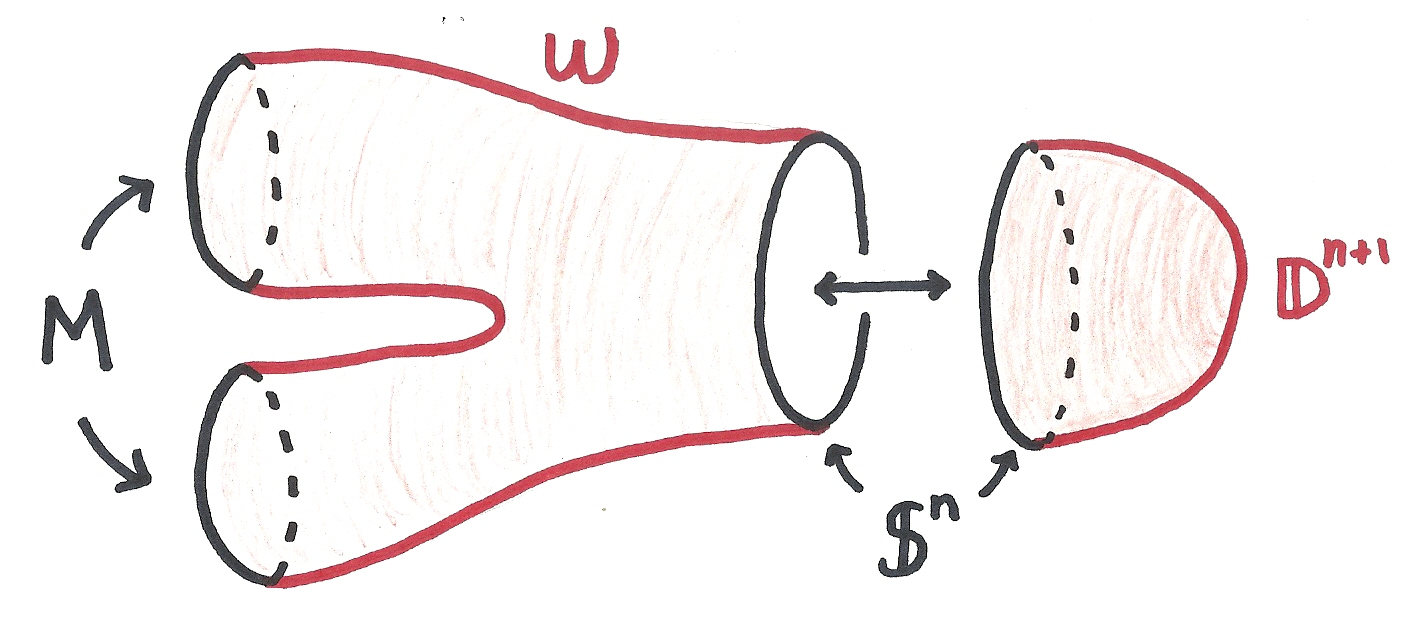
\includegraphics[scale=0.14]{suma_conexa}
    \end{figure}%%%%%%%%%%%%%%%%%%%%%%%%%%%%%%%%%%%%%%%%%%%%%%%%%%%%%%%%%%%%%%%%%%%%%%%%%%%%%%%%%%%
  \item[($\onlyif$)] Sea $N$ la variedad garantizada por hip\'otesis y defino $W=N\sqcup\DD^{n+1}$
    junto con $G:W\ra X$ como $G=F\sqcup \cte$. Observa que
    $\partial W=\partial N\sqcup \partial\DD^{n+1}\cong M\sqcup\Sn^n$. Adem\'as:
    \begin{eqnarray*}
      G|_M&=&G|_{\partial N}=F|_{\partial N}=F|_M=f \\
      G|_{\Sn^n}&=& G|_{\partial\DD^{n+1}}=(G|_{\DD^{n+1}})|_{\partial\DD^{n+1}}=(\cte)|_{\partial\DD^{n+1}}=\cte.
    \end{eqnarray*}
    Por lo tanto $[M,f]=[\Sn^n,\cte]=0$.
  \end{enumerate}
\end{proof}


Observa que si $\varphi:X\ra Y$ es continua, entonces \'este induce un morfismo de grupos
$\varphi_*:\eta_n(X)\ra\eta_N(Y)$ definido por $\varphi_*[M,f]\mapsto[M,\varphi\circ f]$. Entonces
$\eta_n:\cat{Top}\ra\cat{Ab}$ es un funtor:

\import{\directory}{ejercicios/39} %%%%%%%%%%%%%%%%%%%%%%%%%%%%%%%%%%%%%%%%%%%%%%%%%% EJERCICIO 39

\begin{nota}
  Este \'ultimo ejercicio prueba que $X\mapsto\eta_n(X)$ es un funtor entonces preserva isomorfismos,
  es decir:
  \[
    X\approx Y \quad\then\quad \eta_n(X)\cong\eta_n(Y)
  \]
  o en otras palabras, $\eta_n$ es un invariante topol\'ogico.
\end{nota}

De hecho, $\eta_n$ es m\'as que un invariante topol\'ogico, es un invariante homot\'opico. Para
probar esto necesito:

\begin{prop}
  Sean $\varphi,\psi:X\ra Y$ funciones continuas. Entonces $\varphi\simeq\psi\then\varphi_*=\psi_*$.
\end{prop}
\begin{proof}
  Sea $[M,f]\in\eta_n(X)$, entonces $\varphi_*[M,f]=[M,\varphi\circ f]$ y $\psi_*[M,\psi\circ f]$.
  Por hip\'otesis $\varphi\simeq\psi$ mediante alguna homotop\'ia $H:X\times I\ra Y$ (en particular
  $H_0=\varphi$ y $H_1=\psi$). Ahora considera $F:M\times I\ra Y$ definido por la composici'on
  \[
    \begin{tikzcd}
      M\times I \arrow[rr,"f\times\Id"] && X\times I \arrow[rr,"H"] && Y
    \end{tikzcd}.
  \]
  Observa que $F(x,0)=H(f(x),0)=\varphi(f(x))$ y $F(x,1)=H(f(x),1)=\psi(f(x))$, es decir:
  \[
    F|_{M\times\{0\}}=\varphi\circ f \quad\text{y}\quad F|_{M\times\{1\}}=\psi\circ f.
  \]
  Como $\partial(M\times I)=(M\times\{0\})\sqcup(M\times\{1\})=M\sqcup M$ y $F$ es continua, entonces
  $[M,\varphi\circ f]\sim[M,\psi\circ f]$ y as\'i $\varphi_*[M,f]=\psi_*[M,f]$ para toda
  $[M,f]\in\eta_n(X)$.
\end{proof}

\import{\directory}{ejercicios/40} %%%%%%%%%%%%%%%%%%%%%%%%%%%%%%%%%%%%%%%%%%%%%%%%%% EJERCICIO 40

Esta idea se puede generalizar. En lugar de tomar $M^n$ sin frontera para las clases $[M,f]$, puedo
tomar $M$ con frontera tal que $f[\partial M]\subseteq A$ donde $A\subseteq X$ es un conjunto
cerrado fijo. Estas clases se denotan por $\eta_n(X,A)$. Estos grupos son importantes porque
forman una sucesi\'on exacta larga:
\[
  \cdots \lra \eta_n(A) \lra \eta_n(X) \lra \eta_n(X,A) \morf{\delta}
  \eta_{n-1}(A)\lra \eta_{n-1}(X) \lra \cdots
\]
donde $\delta[M,f]=[\partial M,f|_{\partial M}]$. Los grupos $\eta_n(X,A)$ cumplen la propiedad
de \emph{escisi\'on}:

\begin{thm}
  Sea $U\subset A\subseteq X$ tal que $\bar{U}\subseteq\mathring{A}$. Entonces la inclusi\'on
  $\imath:(X-U,A-U)\hookrightarrow (X,A)$ induce un isomorfismo $\eta_n(X-U,A-U)\cong\eta_n(X,A)$.
\end{thm}

En general si $h_*(X,A)=\{h_n(X,A)\}_{n=0}^{\infty}$ es una familia de grupos abelianos tales que
$(X,A)\mapsto h_N(X,A)$ es funtorial, existe una sucesi\'on exacta larga
\[
  \cdots \lra h_n(A) \lra h_n(X) \lra h_n(X,A) \lra h_{n-1}(A)\lra h_{n-1}(X) \lra \cdots
\]
y cada $h_n$ cumple la propiedad de escici\'on, se dice que $h_*(X,A)$ es una teor\'ia de
homolog\'ia.

Ahora calculo $\eta_n$ de un punto. Para esto, denoto $\eta_n:=\eta_n(\{x\})$. Observa que los
elementos de $\eta_n$ son de la forma $[M,\cte]$. Por lo tanto $[M]=[N]$ si y s\'olo si existe
una variedad $W^{n+1}$ y una funci\'on $F:W\ra\{x\}$ continua (ie. $F=\cte$) tal que
$\partial W= M \sqcup N$. Como $F$ es necesariamente constante, dos elementos $[M,\cte]$ y $[N,\cte]$
de $\eta_n$ son iguales si son frontera de una variedad de dimensi\'on $n+1$. Vale la pena mencionar
que si $M=\partial N$ entonces $[M,\cte]=0=[\Sn^n,\cte]$; nada m\'as toma $W=N\sqcup\DD^{n+1}$.


Como todas las funciones en este caso son constantes, denotar\'e a la clase $[M,\cte]\in\eta_n$
simplemente por $[M]$ y se llama la \emph{clase de bordismo de} $M$. Calcular las clases de
bordismo de variedades de dimensi\'on cero es sencillo:

\import{\directory}{ejercicios/41} %%%%%%%%%%%%%%%%%%%%%%%%%%%%%%%%%%%%%%%%%%%%%%%%%% EJERCICIO 41

Para calcular $\eta_1$, s\'olo basta recordar la clasificaci\'on de variedades cerradas de
dimensi\'on 1: si $[M]\in\eta_1$ entonces $M\cong\Sn^1\sqcup\cdots\sqcup\Sn^1$ y as\'i
$[M]=[\Sn^1\sqcup\cdots\sqcup\Sn^1]=[\Sn^1]+\cdots+[\Sn^1]=0+\cdots+0=0$ para toda $[M]\in\eta_1$.
Por lo tanto $\eta_1=0$.

Para dimensi\'on $2$, uso la clasificaci\'on de superficies cerradas: para toda $[M]\in\eta_2$
tengo que $M$ es una suma conexa de toros o una suma conexa de planos proyectivos. En el primer
caso, $M$ es la frontera de ls suma conexa de toros rellena y as\'i $[M]=0$. Por lo tanto
$\eta_2=\ZZ_2$, generado por $[\RR P^2]$.

En general,
\[
  \eta_*:=\bigoplus_{n=0}^{\infty}\eta_n
\]
es un grupo abeliano graduado con graduaci\'on $\eta_n\times\eta_m\ra\eta_{n+m}$ definido por
$([M],[N])\mapsto [M\times N]$.

\begin{thm}(Thom)
  Sean $\{x_2,x_4,x_5,\ldots\}$ variables independientes con sub\'indices $n\neq 2^m-1$ para toda $m$.
  Entonces $\eta_*\cong\ZZ_2[x_2,x_4,x_5,\ldots]$ donde el isomorfismo se puede tomar de tal manera
  que la imagen de $x_n$ es un elemento de $\eta_n$ y que $x_{2n}\mapsto[\RR P^{2n}]$.
\end{thm}

De este teorema se tiene inmediatamente que $\eta_3=0$ porque no hay un polinomio
$\pm x_2\pm x_4\pm x_5\pm\cdots$ que corresponda a un $[M]\in\eta_3$ donde $M$ es de dimensi\'on 3.

\import{\directory}{ejercicios/42} %%%%%%%%%%%%%%%%%%%%%%%%%%%%%%%%%%%%%%%%%%%%%%%%%% EJERCICIO 42

\subsection{Cobordismo con Orientaci\'on}

Hay una teor\'ia similar al cobordismo si incluimos orientaci\'on:

\begin{defin}
  Sobre el conjunto de parejas $((M,\fO_M),f)$, donde $M$ es una variedad cerrada con orientaci\'on
  $\fO_M$ y $f:M\ra X$ es una funci\'on continua, defino la siguiente relaci\'on
  de equivalencia: $((M^n,\fO_M),f)\sim((N^n,\fO_N),g)$ si y s\'olo si
  \[
    \exists F:W^{n+1}\ra X;\;\text{continua tal que}\;\;
    \begin{cases}
      (i)& (\partial W,\fO_{\partial W})\cong (M,\fO_M)\sqcup (N,\fO_N) \\
      (ii)& F|_{M}=f \;\;\text{y}\;\; F|_{N}=g
    \end{cases}
  \]
  donde $W$ es una variedad suave, compacta, con frontera y el difeomorfismo entre las fronteras
  preserva las orientaciones.
\end{defin}

De la misma manera que defin\'i $\eta_n$, defino $\Omega_n$ como las clases $[(M,\fO_M),f]$ sobre
$X=\{x\}$. En este caso, $\Omega_0$ tambi\'en son 0-variedades compactas, ie. conjuntos finitos
pero como tambi\'en est\'an orientadas, cada punto viene con un signo. Por ejemplo si $M=\{x_1,x_2\}$
entonces una orientaci\'on de $M$ puede ser $(M,\fO_M)=\{(x_1,-1),(x_2,+1)\}$.

M\'as precisamente, si $M=\{x_1,\ldots,x_n\}$ es una variedad compacta de dimensi\'on 0, una
orientaci\'on $\fO_M$ es un conjunto $\{\fo_1,\ldots,\fo_n\}$ donde $\fo_j\in\{-1,+1\}$. Entonces
la variedad orientada se escribe como $(M,\fO_M)=\{(x_j,\fo_j)\}$. Por lo tanto puedo reordenar
los elementos de $M$ tal que aparecen primero los que tienen orientaci\'on positiva. Es decir,
puedo escribir $M=\{x_1,\ldots,x_m,x_{m+1},\ldots,x_{m+m'}\}$ donde $\fo_j=+1$ para $j\in\{1,\ldots,m\}$
y $\fo_{m+j}=-1$ para $j\in\{1,\ldots,m'\}$.

Ahora me pregunto cuando $(M,\fO_M)$ es la frontera de una 1-variedad orientada $(W,\fO_W)$.
Primero observa que toda 1-variedad compacta es la uni\'on disjunta (finita) de
intervalos/trayectorias y c\'irculos, pero como s\'olo me interesa la frontera de $W$ y
$\partial\Sn^1=\emptyset$, puedo considerar solamente las $W$ cuyas componentes son unicamente
intervalos/trayectorias (sin ser lazos). Adem\'as puedo asumir que $W$ est\'a encajado en alg\'un
$\RR^N$ entonces s\'i puedo asumir que los componentes de $W$ efectivamente son trayectorias,
ie. im\'agenes suaves del intervalo $[0,1]$.

En este caso, $\partial W$ es la uni\'on disjunta de los puntos iniciales y finales de cada
componente de $W$. Adem\'as ning\'un punto en $\partial W$ puede estar en dos trayectorias
distintas ya que sucede uno de dos casos prohibidos: las trayectorias se intersectan y producen
una variedad no diferenciable; el punto es inicial de una trayectoria y final de otra trayectoria
que se pegan suavemente, pero en este caso este punto no est\'a en $\partial W$. Por lo tanto
cada pareja de elementos distintos de $\partial W$ est\'an conectados por una \'unica
trayectoria en $\RR^N$ que es una componente abierta de $W$.
Adem\'as, una orientaci\'on de $W$ induce una orientaci\'on en $\partial W$: simplemente le asigna
un $-1$ a los puntos iniciales y un $+1$ a los puntos finales.
Para aclarar esta discusi\'on, considera la figura \ref{fig:frontera_1variedad_orientada} %
%
\begin{figure}[ht] %%%%%%%%%%%%%%%%%%%%%%%%%%%%%%%%%%%%%%%%%%%%% FIGURA FRONTERA_1VARIEDAD_ORIENTADA
  \centering\caption{$\;$}\label{fig:frontera_1variedad_orientada}
  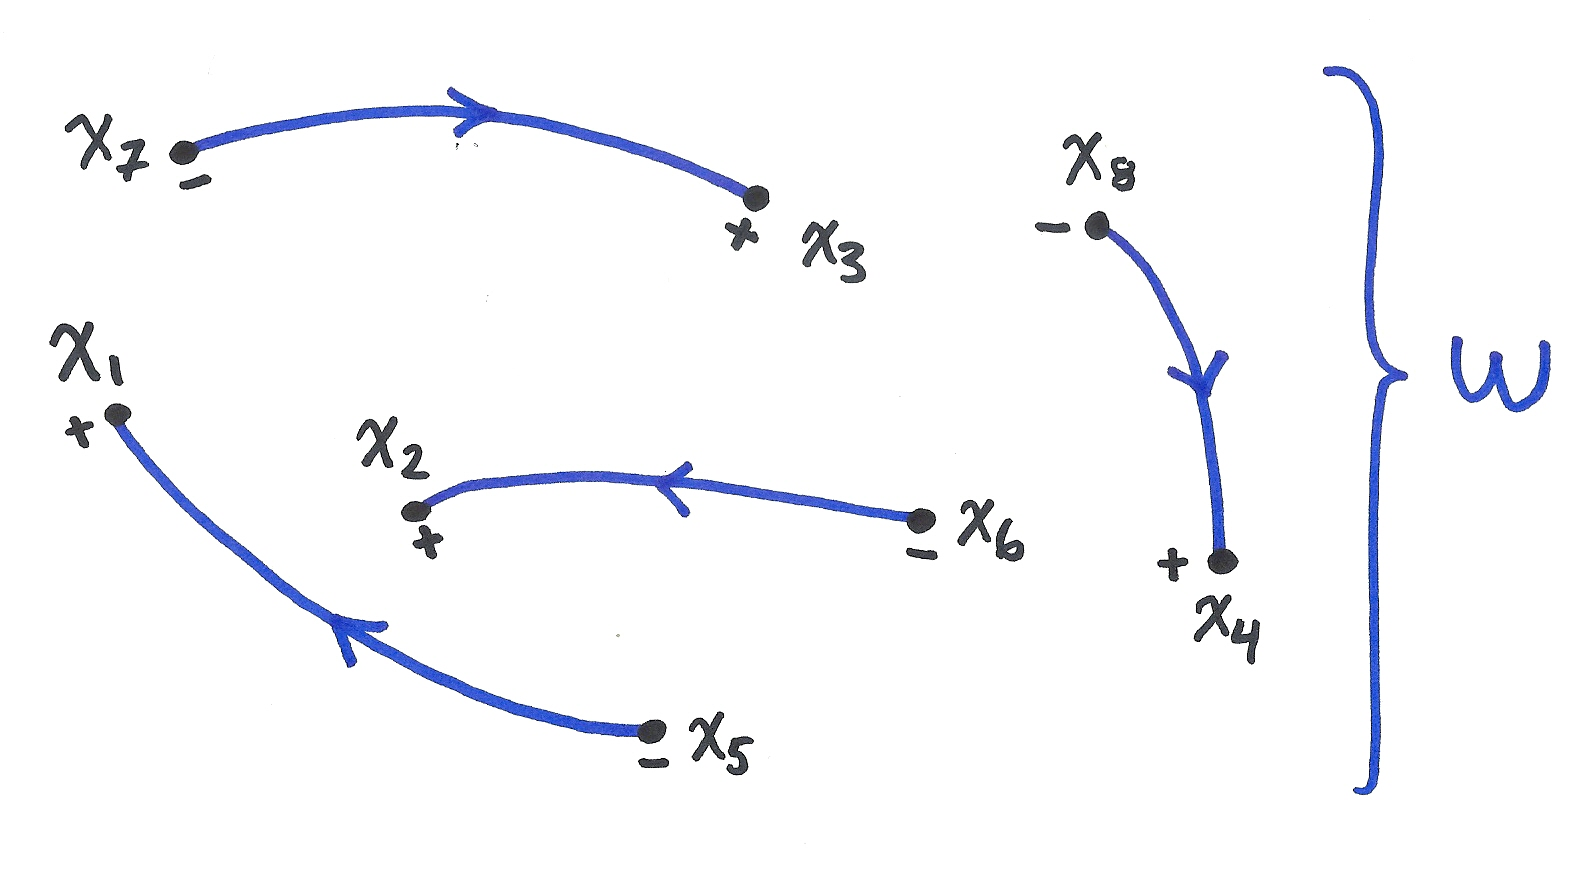
\includegraphics[scale=0.12]{frontera_1variedad_orientada}
\end{figure}%%%%%%%%%%%%%%%%%%%%%%%%%%%%%%%%%%%%%%%%%%%%%%%%%%%%%%%%%%%%%%%%%%%%%%%%%%%%%%%%%%%%%%%
%
donde la frontera de $W$ es
\[
  (\partial W,\fO_{\partial W})=
  \{(x_1,+1),(x_2,+1),(x_3,+1),(x_4,+1),(x_5,-1),(x_6,-1),(x_7,-1),(x_8,-1)\}
\]

Observa que si $(M,\fO_M)$ es la frontera de la 1-variedad orientada $(W,\fO_W)$ entonces
$M$ tiene la misma cantidad de puntos orientados positivamente que de puntos orientados negativamente;
ya que las trayectorias inducen una biyecci\'on entre los puntos iniciales (ie. los puntos orientados
negativamente) y los puntos finales (ie. los puntos orientados positivamente). En particular
tengo:

\begin{prop}\label{prop:cantidad_orientaciones}
  Si $(M,\fO_M)$ es una 0-variedad cerrada tal que $(M,\fO_M)\cong(\partial W,\fO_{\partial W})$,
  donde el difeomorfismo preserva orientaci\'on, entonces
  \[
    \#\{x\in M\mid \fo_x=+1\}=\#\{x\in M\mid \fo_x=-1\}.
  \]
\end{prop}

M\'as generalmente tengo:

\import{\directory}{ejercicios/43} %%%%%%%%%%%%%%%%%%%%%%%%%%%%%%%%%%%%%%%%%%%%%%%%%%% EJERCICIO 43

\end{document}